\documentclass[a4paper,14pt]{extarticle}

% Путь до папки с общими шаблонами
\newcommand{\pathToCommonFolder}{/home/denilai/Desktop/LaTeX/Common}
% Название работы в титуле
\newcommand{\workname}{Отчет по практической работе №3}
% Название дисциплины в титуле
\newcommand{\discipline}{Системное программное обеспечение}
% Название кафедры в титуле
\newcommand{\kafedra}{Кафедра Математического обеспечения и стандартизации информационных технологий}
% Тема работы в титуле
\newcommand{\theme}{Docker}
\newcommand{\rang}{ассистент}
\newcommand{\teacherfio}{Ю.~А.~Вороноцов}



% установка размера шрифта для всего документа
%\fontsize{20pt}{18pt}\selectfont
\usepackage{extsizes} % Возможность сделать 14-й шрифт

\author{Кирилл Денисов}
\title{Практическая работа №3}
\date{\today}

% установка полуторного интервала
% \usepackage{setspace}  
% \onehalfspacing

% использовать Times New Roman
\renewcommand{\rmdefault}{ftm}

% Вставка заготовки преамбулы
% Этот шаблон документа разработан в 2014 году
% Данилом Фёдоровых (danil@fedorovykh.ru) 
% для использования в курсе 
% <<Документы и презентации в \LaTeX>>, записанном НИУ ВШЭ
% для Coursera.org: http://coursera.org/course/latex .
% Исходная версия шаблона --- 
% https://www.writelatex.com/coursera/latex/5.3

% В этом документе преамбула

% Для корректного использования русских символов в формулах
% пакеты hyperref и настройки, связанные с ним, стоит загуржать
% перед загрузкой пакета mathtext



% поддержка русских букв
% кодировка шрифта
%\usepackage[T2A]{fontenc} 
\usepackage{pscyr}

% использование ненумеровонного абзаца с добавлением его в содержаниеl

\newcommand{\anonsection}[1]{\section*{#1}\addcontentsline{toc}{section}{#1}}
\newcommand{\sectionunderl}[1]{\section*{\underline{#1}}}


% настройка окружения enumerate
\usepackage{enumitem}
\setlist{noitemsep}
\setlist[enumerate]{labelsep=*, leftmargin=1.5pc}

\usepackage{hyperref}

% сначала ставить \usepackage{extsizes} % Возможность сделать 14-й шрифт
% для корректной установки полей вставлять преамбулу следует в последнюю очередь (но перед дерективой замены \rmdefault)
\usepackage[top=20mm,bottom=25mm,left=35mm,right=20mm]{geometry} % Простой способ задавать поля

\hypersetup{				% Гиперссылки
	unicode=true,           % русские буквы в раздела PDF
	pdftitle={Заголовок},   % Заголовок
	pdfauthor={Автор},      % Автор
	pdfsubject={Тема},      % Тема
	pdfcreator={Создатель}, % Создатель
	pdfproducer={Производитель}, % Производитель
	pdfkeywords={keyword1} {key2} {key3}, % Ключевые слова
	colorlinks=true,       	% false: ссылки в рамках; true: цветные ссылки
	linkcolor=red,          % внутренние ссылки
	citecolor=black,        % на библиографию
	filecolor=magenta,      % на файлы
	urlcolor=blue           % на URL
}

%%% Работа с русским языком
\usepackage{cmap}					% поиск в PDF
\usepackage{mathtext} 				% русские буквы в формулах
\usepackage[T2A]{fontenc}			% кодировка
\usepackage[utf8]{inputenc}			% кодировка исходного текста
\usepackage[english,russian]{babel}	% локализация и переносы
\usepackage{indentfirst}
\frenchspacing

%для изменения названия списка иллюстраций
\usepackage{tocloft}


\renewcommand{\epsilon}{\ensuremath{\varepsilon}}
\renewcommand{\phi}{\ensuremath{\varphi}}
\renewcommand{\kappa}{\ensuremath{\varkappa}}
\renewcommand{\le}{\ensuremath{\leqslant}}
\renewcommand{\leq}{\ensuremath{\leqslant}}
\renewcommand{\ge}{\ensuremath{\geqslant}}
\renewcommand{\geq}{\ensuremath{\geqslant}}
\renewcommand{\emptyset}{\varnothing}

% Изменения параметров списка иллюстраций
\renewcommand{\cftfigfont}{Рисунок } % добавляем везде "Рисунок" перед номером
\addto\captionsrussian{\renewcommand\listfigurename{Список иллюстративного материала}}

\newcommand{\tm}{\texttrademark\ }
\newcommand{\reg}{\textregistered\ }


%%% Дополнительная работа с математикой
\usepackage{amsmath,amsfonts,amssymb,amsthm,mathtools} % AMS
\usepackage{icomma} % "Умная" запятая: $0,2$ --- число, $0, 2$ --- перечисление

%% Номера формул
%\mathtoolsset{showonlyrefs=true} % Показывать номера только у тех формул, на которые есть \eqref{} в тексте.
%\usepackage{leqno} % Нумереация формул слева

%% Свои команды
\DeclareMathOperator{\sgn}{\mathop{sgn}}

%% Перенос знаков в формулах (по Львовскому)
\newcommand*{\hm}[1]{#1\nobreak\discretionary{}
{\hbox{$\mathsurround=0pt #1$}}{}}


% отступ для первого абзаца главы или параграфа
%\usepackage{indentfirst}

%%% Работа с картинками
\usepackage{graphicx}  % Для вставки рисунков
\graphicspath{{images/}{screnshots/}}  % папки с картинками
\DeclareGraphicsExtensions{.pdf,.png,.jpg}
\setlength\fboxsep{3pt} % Отступ рамки \fbox{} от рисунка
\setlength\fboxrule{1pt} % Толщина линий рамки \fbox{}
\usepackage{wrapfig} % Обтекание рисунков текстом

%%% Работа с таблицами
\usepackage{array,tabularx,tabulary,booktabs} % Дополнительная работа с таблицами
\usepackage{longtable}  % Длинные таблицы
\usepackage{multirow} % Слияние строк в таблице

%%% Теоремы
\theoremstyle{plain} % Это стиль по умолчанию, его можно не переопределять.
\newtheorem{theorem}{Теорема}[section]
\newtheorem{proposition}[theorem]{Утверждение}

\theoremstyle{plain} % Это стиль по умолчанию, его можно не переопределять.
\newtheorem{work}{Практическая работа}[part]


 
 
\theoremstyle{definition} % "Определение"
\newtheorem{corollary}{Следствие}[theorem]
\newtheorem{problem}{Задача}[section]
 
\theoremstyle{remark} % "Примечание"
\newtheorem*{nonum}{Решение}



%%% Программирование
\usepackage{etoolbox} % логические операторы

%%% Страница

%	\usepackage{fancyhdr} % Колонтитулы
% 	\pagestyle{fancy}
%   \renewcommand{\headrulewidth}{0pt}  % Толщина линейки, отчеркивающей верхний колонтитул
% 	\lfoot{Нижний левый}
% 	\rfoot{Нижний правый}
% 	\rhead{Верхний правый}
% 	\chead{Верхний в центре}
% 	\lhead{Верхний левый}
%	\cfoot{Нижний в центре} % По умолчанию здесь номер страницы

\usepackage{setspace} % Интерлиньяж
\onehalfspacing % Интерлиньяж 1.5
%\doublespacing % Интерлиньяж 2
%\singlespacing % Интерлиньяж 1

\usepackage{lastpage} % Узнать, сколько всего страниц в документе.

\usepackage{soul} % Модификаторы начертания


\usepackage[usenames,dvipsnames,svgnames,table,rgb]{xcolor}


\usepackage{csquotes} % Еще инструменты для ссылок

%\usepackage[style=authoryear,maxcitenames=2,backend=biber,sorting=nty]{biblatex}

\usepackage{multicol} % Несколько колонок

\usepackage{tikz} % Работа с графикой
\usepackage{pgfplots}
\usepackage{pgfplotstable}

% модуль для вставки рыбы
\usepackage{blindtext}

\usepackage{listings}
\usepackage{color}


% для поворота отдельной страницы. Использовать окружение \landscape
\usepackage{pdflscape} 
\usepackage{rotating} 


\definecolor{mygreen}{rgb}{0,0.6,0}
\definecolor{mygray}{rgb}{0.5,0.5,0.5}
\definecolor{mymauve}{rgb}{0.58,0,0.82}


% пример импорта файла
%\lstinputlisting{/home/denilai/repomy/conf/distributions}

\lstset{
	language=Python,
	basicstyle=\footnotesize,        % the size of the fonts that are used for the code
	numbers=left,                    % where to put the line-numbers; possible values are (none, left, right)
	numbersep=5pt,                   % how far the line-numbers are from the code
	numberstyle=\tiny\color{mygray}, % the style that is used for the line-numbers
	stepnumber=2,                    % the step between two line-numbers. If it's 1, each line will be numbered
	% Tab - 2 пробела
	tabsize=2,    
	% Автоматический перенос строк
	breaklines=true,
	frame=single,
	breakatwhitespace=true,
	title=\lstname 
}



\begin{document}
	\thispagestyle{empty}
	
	% Вставка первого титульного листа
	%\newcounter{withouttheme}

%\setcounter{withouttheme}{<n>} установить значение счетчика  withouttheme для определения, нужна ли тема
%    {0} - нужна
%    {1} - не нужна

%\setcounter{withoutsubmissiondate}{<n>} установить значение счетчика  withoutsubmissiondate для определения, нужна ли дата представления к защите
%     {0} - нужна
%     {1} - не нужена
\begin{center}
	\begin{figure}[h!]
		\begin{center}
		%\vspace{-10ex}
		
\includegraphics[width=0.17\linewidth]{\pathToCommonFolder/gerb}
		%\caption{}\label{pic:first}
		%	\vspace{5ex}
		\end{center}	
	\end{figure}
 	\small	МИНОБРНАУКИ РОССИИ \\
	Федеральное государственное бюджетное образовательное учреждение\\
						высшего образования\\
\normalsize					
\textbf{«МИРЭА – Российский технологический университет»\\
						РТУ МИРЭА}\\
						\noindent\rule{1\linewidth}{1pt}\\
       Институт информационных технологий\\ %\vspace{2ex}
					\kafedra\\
		\vspace{3ex}
			\large \textbf{\workname}  \\
		%\vspace{1ex}
						по дисциплине\\ «\discipline» \\
		\vspace{3ex}
		\ifnum \value{withouttheme}=0 {
			\textbf{Тема работы:}\\ <<\theme>>
		}
		\else {}
		\fi
\vspace{10ex}
\small
\begin{table}[h!]
\begin{tabular}{lp{0.6\linewidth}l}
	\textbf{Выполнил:} & студент группы ИВБО-02-19 & \\ 
	& & \studentfio \\%Д.~Н.~Федосеев\\%А.~М.~Сосунов\\%К.~Ю.~Денисов\\%И.~А.~Кремнев
	\textbf{Принял:} & \rang & \\
	& & \teacherfio \hfill\\
\end{tabular}
\end{table}
\end{center}
\ifnum \value{withoutsubmissiondate}=0 {
	\begin{flushleft}
		Работа представлена к защите <<\rule{3ex}{1pt}>>\rule{10ex}{1pt} 202\rule{1ex}{1pt} г.\hfill
	\end{flushleft}
\else {}
\fi

\normalsize
\begin{center}	
\vfill
Москва 2022
\end{center}

	
	\newpage
	\tableofcontents
	\newpage

\section{Ход работы}
В ходе данной практической работы будет рассмотрена работа с пакетным менеджером \textit{apt} в операционной системе Ubuntu Linux.
\subsection{Установка нового пакета}
После выполнения команд в терминале
\begin{lstlisting}
	$ sudo apt-get install mc
	$ sudo apt-get install htop
	$ sudo apt-get install neofetch
\end{lstlisting}
на машину будут установлены соответствующие пакеты.
\subsection{Удаление пакета}
Для удаления пакета neofetch без удаления конфигурационных файлов следует использовать команду 
\begin{lstlisting}
$ sudo apt-get remove neofetch
\end{lstlisting}

При использовании такой команды в системе остаются конфигурационные файлы программы, а также дополнительные пакеты. Чтобы удалить конфигурационные файлы можно использовать опцию --purge или команду purge:
\begin{lstlisting}
$ sudo apt-get --purge remove neofetch
\end{lstlisting}
\subsection{ Поиск пакета и вывод информации о нем}
Для поиска пакета \textit{sqlite} третьей версии в дереве репозиториев и вывода информации о нем, следует использовать нижеуказанные команды:
\begin{lstlisting}
$ sudo apt-cache pkgnames 
$ sudo apt-cache show sqlite3
\end{lstlisting}

В результате выполнения этих команд мы получим подробную информацию о пакете. См рисунок \ref{img:apt-cache}

\begin{figure}[h!]
	\centering
	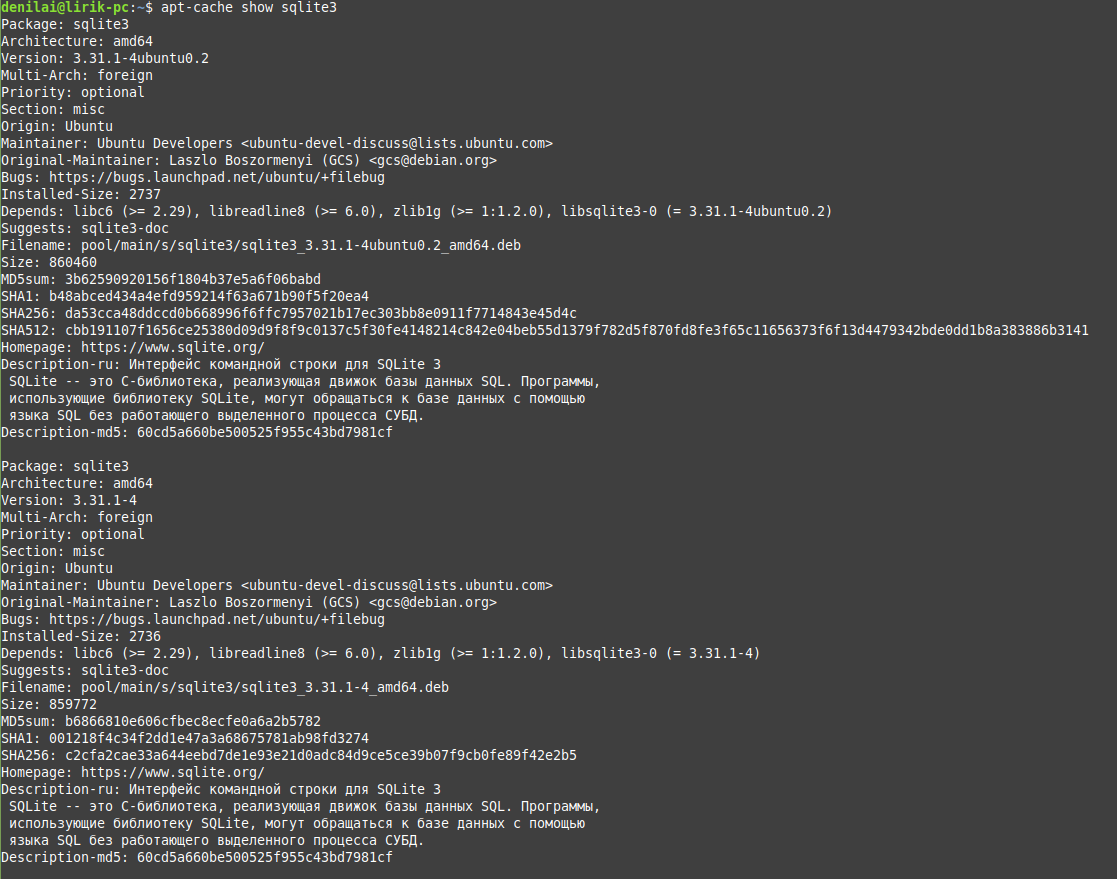
\includegraphics[width=0.9\linewidth]{apt-cache}
	\caption{Поиск пакета в дереве репозиториев}
	\label{img:apt-cache}
\end{figure}

\section{Добавление репозиториев}
Ознакомимся с командами, необходимыми для добавления репозитория Postgresql:
\begin{lstlisting}
	$ sudo sh -c 'echo "deb http://apt.postgresql.org/pub/repos/apt/ `lsb_release -cs`-pgdg main" >> /etc/apt/sources.list.d/pgdg.list'
	$ wget -q https://www.postgresql.org/media/keys/ACCC4CF8.asc -O - | sudo apt-key add -
	$ sudo apt-get update
	$ sudo apt install postgresql postgresql-contrib
\end{lstlisting}
Что содержится в командах:
\begin{enumerate}
	\item Добавляется репозиторий в список репозиториев apt (добавление строчки в sources.list)
	\item Загружается ключ репозитория и добавляется в пакетный менеджер
	\item Обновляется список пакетов
	\item Установка пакета
\end{enumerate}
В общем случае может быть более простой способ:
\begin{lstlisting}
	$ sudo add-apt repository ppa:repo/ppa
\end{lstlisting}
После ознакомления с примерами, установим docker, следуя рекомендациям, приведенным в официальной \href{https://docs.docker.com/engine/install/debian/}{документации}.
\newpage
\section{Сборка пакетов из исходных кодов}
В общем случае сборка пакетов выглядит следующим образом:
\begin{enumerate}
	\item Загрузка архива с исходным кодом (чаще всего .tar.gz)
	\item Разархивирование (либо в ui, либо см. tar и его использование)
	\item  Переход в директорию
	\item ./configure
	\item make
	\item sudo make install
\end{enumerate}
Загрузим архив с исходными кодами программы sqlite и установим ее в систему в соответствии с вышеуказанными действиями. См рисунки в \hyperref[A]{Приложении А}.
\section{Создание собственного deb-пакета}
\subsection{Подготовка окружения}
\begin{enumerate}
	\item В качестве скрипта, который будет помещен в пакет, выберем скрипт $parseawk.sh$, который был написан в ходе первой практической работы по дисциплине "Системное программное обеспечение".
	\item Установим необходимые пакеты для сборки пакетов
	\begin{lstlisting}
	$ sudo apt-get install dpkg debconf debhelper lintian
	\end{lstlisting}
	\item Создадим такую структуру папок, содержащих файлы, необходимые для создания deb-пакета. См. рисунок \ref{img:struct}. Файлы в структуре выделены цветом.
	\begin{figure}[h!]
		\centering
		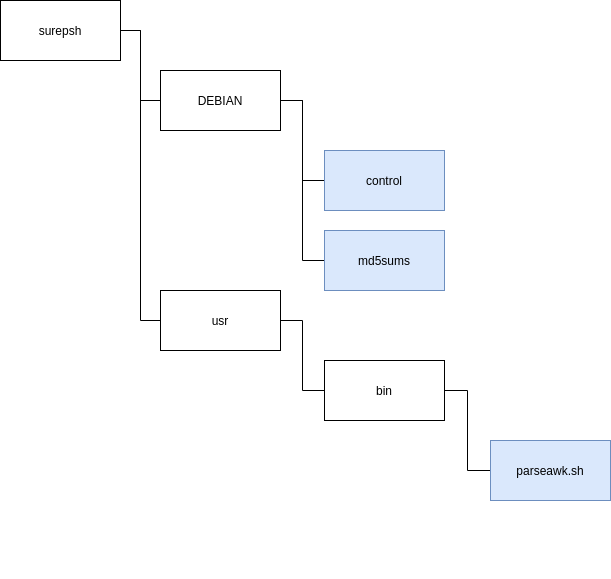
\includegraphics[width=0.6\linewidth]{supersh-struct}
		\caption{Структура директории supersh}
		\label{img:struct}
		\end{figure}
\end{enumerate}
\subsection{Описание пакетирования}
Создадим файл $control$ --- цельный файл пакета, описывающий все основные свойства в виде пары <<Атрибут: Значение>>. Заполним необходимые атрибуты.
%\begin{lstlisting}[~supersh/DEBIAN/control]
\lstinputlisting{/home/denilai/supersh/DEBIAN/control}

Этого файла достаточно для создания работоспособного пакета. После заполнения файла $control$ следует приступить к сборке пакета.
\subsection{Сборка пакета}
Первое, что нужно сделать --- это рекурсивно выставить всем файлам в корне пакета пользователя и
группу root:root (или другие, если потребуется). Это нужно затем, что файлы пакета упаковываются в
tar.gz архив который сохраняет и права доступа к файлам, и владельца. Выполним команду
\begin{lstlisting}
$ sudo chmod -R root:root
\end{lstlisting}

Как альтернативу данной команде следует упомянуть $fakeroot$. Данная утилита позволяет запускать программы в Linux с привилегиями суперпользователя для выполнения любых файловых операций. Изменения видны только для запущенной под fakeroot программы, реально в системе ничего не меняется, т.е. для программы создается некая виртуальная оболочка, в которой отражаются все действия.
Выполним команду.
\begin{lstlisting}
$ fakeroot dpkg-deb --build supersh
\end{lstlisting}

Созданный пакет необходимо переименовать, чтобы он соответствовал порядку именования *.deb
пакетов:\\<имя пакета><версия><архитектура>.deb.  См. рисунок \ref{img:parseawk-package}.
\begin{lstlisting}
$ mv supersh.deb supersh_1.0-1_all.deb
\end{lstlisting}
\begin{figure}[hpbt]
	\centering
	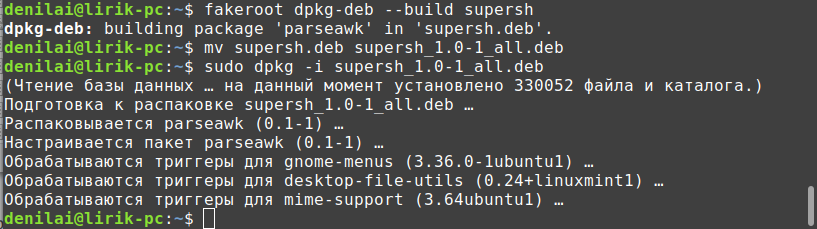
\includegraphics[width=0.8\linewidth]{parseawk-package}
	\caption{Сборка пакета}
	\label{img:parseawk-package}
\end{figure}

\subsection{Установка пакета}
Установим в систему собранный пакет с помощью команды. См. рисунок \ref{img:parseawk-package}.
\begin{lstlisting}
$ sudo dpkg -i supersh_1.0-1_all.deb
\end{lstlisting}

Пользовательский deb-пакет успешно установлен в систему. Скрипт расположен по пути /usr/bin, в соответствии со структурой директорий, указанной при создании пакета.
\section{Создание и настройка\\локального deb-репозитория}
Теперь у нас есть собственный пакет. Когда их будет несколько, и тем более — с зависимостями,
окажется, что намного удобнее быстренько поднять собственный локальный микро-репозиторий, и
включить его в список источников менеджера пакетов. Сперва установим помощника командой 
\begin{lstlisting}
$ sudo apt-get install reprepro
\end{lstlisting}

Затем создадим директорию нашего локального репозитория. Она будет корневой. Создаем файл conf/distributions, который заполняем следующим образом.
\lstinputlisting{/home/denilai/repomy/conf/distributions}
Репозиторий описан. Необходимо создать шаблон репозитория по заданному описанию. Для этого воспользуемся следующими командами:
\begin{lstlisting}
$ reprepro export
$ reprepro createsymlinks
\end{lstlisting}

Следующим шагом необходимо добавить репозиторий в /etc/apt/sources.list, указав такую строку

\begin{lstlisting}
	deb file:///home/denilai/repomy/ karmic soft games
\end{lstlisting}

Для управления пакетами в репозитории поместим *.deb файл в корневую папку репозитория, и добавляем их в компоненту soft дистрибутива karmic с помощью команды
\begin{lstlisting}
reprepro -C soft includedeb karmic *.deb
\end{lstlisting}

Удаление пакетов доступно с помощью команды
\begin{lstlisting}
reprepro -C soft remove karmic supersh
\end{lstlisting}
\begin{figure}[hpbt]
	\centering
	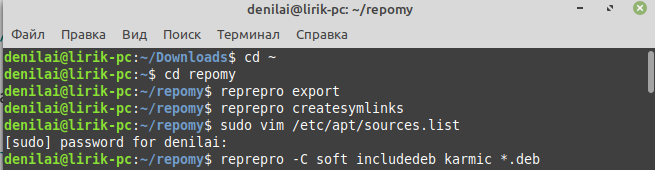
\includegraphics[width=0.9\linewidth]{repo}
	\caption{Работа с репозиторием}
	\label{img:repo}
\end{figure}
\newpage
{\centering
\anonsection{ПРИЛОЖЕНИЕ А}
}
\label{A}
\begin{figure}[hptb]
	\centering
	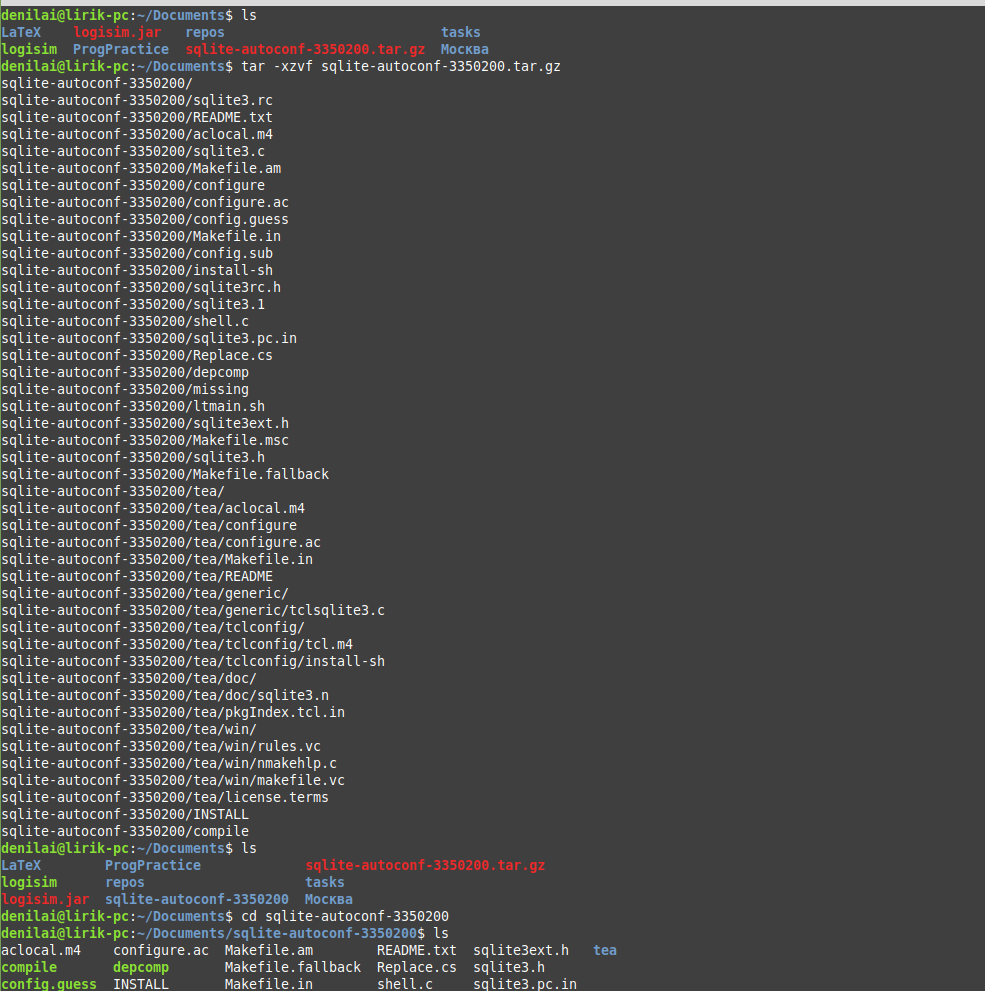
\includegraphics[width=0.9\linewidth]{sqlite-unzip}
	\caption{Разархивирование файла}
	\label{img:sqlite-unzip}
\end{figure}
\begin{figure}[hpbt]
	\centering
	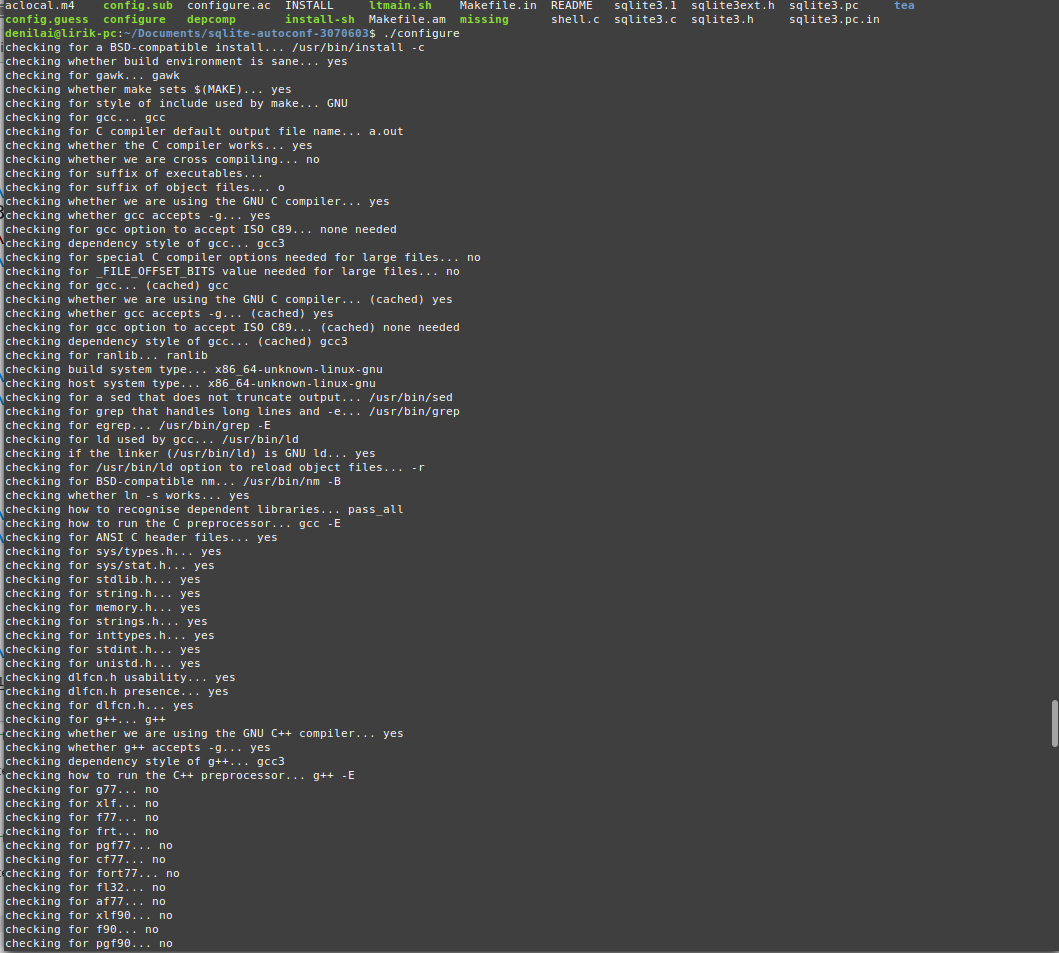
\includegraphics[width=0.9\linewidth]{sqlite-config}
	\caption{Запуск файла config}
	\label{img:sql-config}
\end{figure}

\begin{figure}[htpb]
	\centering
	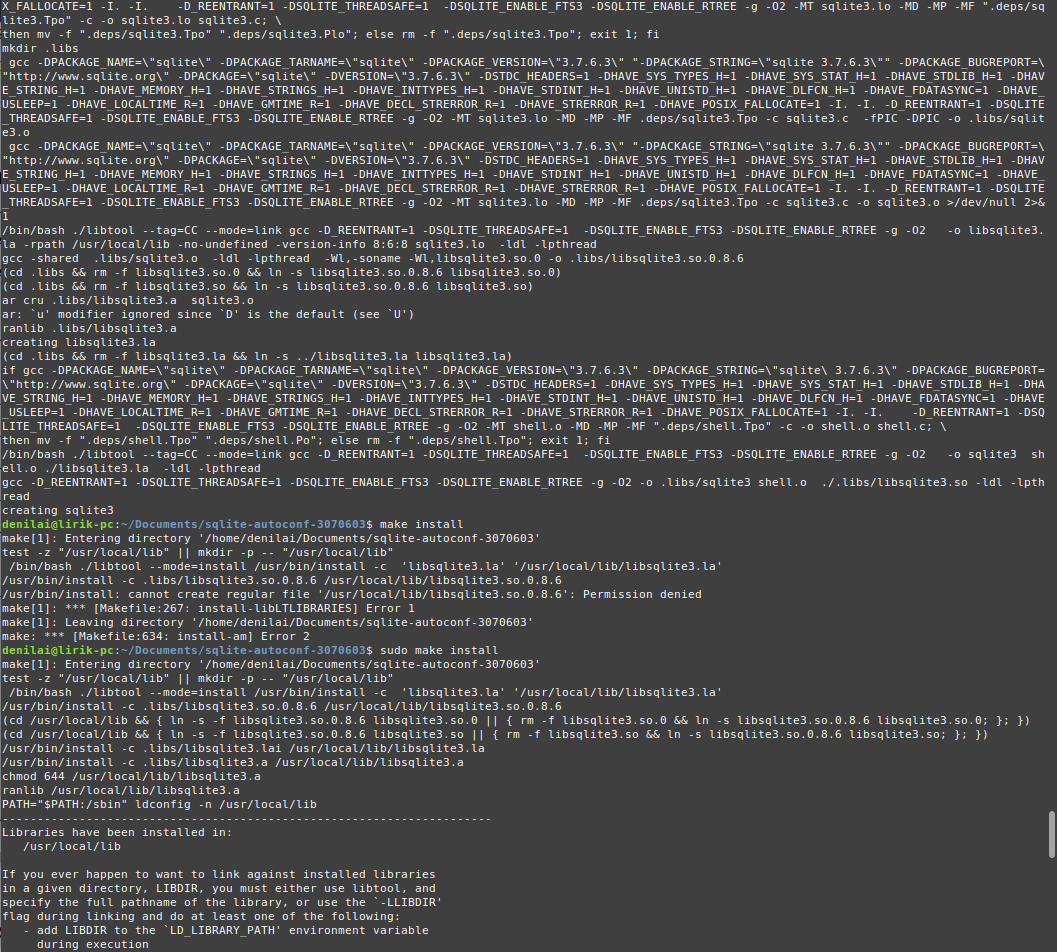
\includegraphics[width=0.9\linewidth]{sqlite-make}
	\caption{Процесс сборки командой make}
	\label{img:sqlite-make}
\end{figure}


\end{document}
